\documentclass[wide,a4paper,titlepage,12pt]{mwart}
\usepackage{polski,graphicx,pdflscape}
\usepackage[utf8]{inputenc}
\usepackage{listings}


\title{Próbkowanie i kwantowanie}
\author{Tymon Tobolski (181037)\\ Jacek Wieczorek (181043)}

% Title page layout (fold)
\makeatletter
\renewcommand{\maketitle}{
\begin{titlepage}
  \begin{center}
    \vspace*{3cm}
    \LARGE \@title \par
    \vspace{2cm}
    \textit{\small Autor:}\par
    \normalsize \@author\par \normalsize
    \vspace{3cm}
    \textit{\small Prowadzący:}\par
    Dr inż. Paweł Biernacki \par
    \vspace{2cm}
    Wydział Elektroniki\\ II rok\\ WT/TN 13:15--15:00 \par
    \vspace{5cm}
    \small \@date
  \end{center}
\end{titlepage}
}
\makeatother
% Title page layout (end)

\begin{document}
  \maketitle
  \section{Cel ćwiczenia} % (fold)
  \label{sec:Cel}
    Celem ćwiczenia jest analiza porcesu próbkowania i kwantyzacji sygnałów okresowych.
    
  \section{Algorytm przetwarzający}
    Wykorzystane funkcje:
    \newline
    \begin{itemize}
      \item generujące sygnał (\textbf{sinus}, \textbf{prostokat}, \textbf{trojkat})
			\item wyznaczająca widmo (\textbf{fftg})
    \end{itemize}
  
  \lstset{ %
    language=Octave,                % choose the language of the code
    basicstyle=\scriptsize,       % the size of the fonts that are used for the code
    numbers=left,                   % where to put the line-numbers
    numberstyle=\scriptsize,      % the size of the fonts that are used for the line-numbers
    stepnumber=10,                   % the step between two line-numbers. If it's 1 each line 
                                    % will be numbered
    numbersep=9pt,                  % how far the line-numbers are from the code
    % backgroundcolor=\color{white},  % choose the background color. You must add \usepackage{color}
    showspaces=false,               % show spaces adding particular underscores
    showstringspaces=false,         % underline spaces within strings
    showtabs=false,                 % show tabs within strings adding particular underscores
    % frame=single,                 % adds a frame around the code
    % tabsize=2,                  % sets default tabsize to 2 spaces
    % captionpos=b,                   % sets the caption-position to bottom
    breaklines=true,                % sets automatic line breaking
    % breakatwhitespace=false,        % sets if automatic breaks should only happen at whitespace
    % title=\lstname,                 % show the filename of files included with \lstinputlisting;
                                    % also try caption instead of title
    % escapeinside={\%*}{*)},         % if you want to add a comment within your code
    % morekeywords={*,...}            % if you want to add more keywords to the set
    }
    \lstinputlisting{lab3.m}
    
  % section Wstęp (end)
  
  \section{Próbkowanie sygnału sinus}
		Badany sygnał został określony następującymi parametrami:
		
		$A=1, f=1000, faza=0, T=1$
				
		\subsection{Częstotliwość próbkowania $fpr > 2f, fpr=10000$}
			Wykresy znajdują się na stronie \pageref{prob1}.
			
		\subsection{Częstotliwość próbkowania $fpr=2f, fpr=2000$}
			Wykresy znajdują się na stronie \pageref{prob2}.
				
		\subsection{Częstotliwość próbkowania $fpr < f, fpr=490$}
			Wykresy znajdują się na stronie \pageref{prob3}.
		
		\subsection{Wnioski}
		Sygnał spróbkowany z częstotliwością $fpr>>f$ w pkt 3.1, odzwierciedla realny przebieg sygnału sinusoidalnego.
		
		W pkt 3.2 spróbkowany sygnał przestawia w przybliżeniu sygnał ciągły o wartości równej 0. Spowodowane jest to tym, iż próbkowanie następuje tylko raz na dwa okresy sygnału, za każdym razem przybierając taką samą wartość.
		
		W pkt 3.3 spróbkowany sygnał przedstawia równeiż sinusoidę, lecz o innej częśtotliwości. Jej wartość nie jest prawdziwa, ze względu na nie zachowania warunków twierdzenia Kotelnikowa - Shannona dotyczących próbkowania, gdzie $fpr > 2*f$. Zachodzi zjawisko aliasingu : niejednożnaczność w dziedzinie częstotliwości. Nieskończenie wiele przebiegów sinusoidalnych pasuje do podanego zestawu próbek. Z takeigo zestawu próbek nie da się otworzyć oryginalnego sygnału, nie jesteśmy wstanie odróżnić sygnału $f$ od $f + k*fpr$.

  \section{Kwantowanie}
		Badana rozdzielczość (ilość bitów przetwornika) $n \in \left \{1, 2, 4, 10\right \}$
		\subsection{Sygnał sinus}
			Badany sygnał został określony następującymi parametrami:
			
			$A=1, f=10, fpr=500, faza=0, T=1$
			\par
			Wraz ze wzrtostem współczynnika $n$, liniowe odwzorowanie sygnału coraz bardziej przypomina sinusoidę, a błąd kwantyzacji maleje. Dzieje się dlatego, że zwiększajać parametr n, zwiększamy tak na prawdę liczbę bitów w przetworniku AC. Kolejne próbki sygnału przypisywane są donajbliższego poziomu reprezentacji. Im większa jest liczba bitów, tym liczba poziomów kwantyzacji też jest większa. Błąd kwantyzacji, jest to różnica pomiędzy wartośćią próbki, a jej poziomem reprezentacji. Wraz ze wzrostem liczby bitów, błąd maleje. Kwantyzacja ma również wpływ na widmo sygnału. W wyniku kwantowania, do widma amplitudowego dodane zostają pewne składowe, wynikające z niedokładności odworowania, cechującego sygnał skwantowany. Im wyzszy poziom kwantyzacji, tym odwzorowanie widma jest dokładniejsze.
			\par
			Wykresy znajdują się na stronach \pageref{kwant1-1}, \pageref{kwant1-2}, \pageref{kwant1-4} i \pageref{kwant1-10}.

		\subsection{Sygnał prostokątny}
			Badany sygnał został określony następującymi parametrami:
			
			$A=1, f=10, fpr=500, faza=0, T=1$
			\par
			Dla sygnału porstokątnego szum kwantyzacji jest równy zero dal wszystkich wartości współczynnika n. Dzieje się to dal tego, że sygnał ten przyjmuje tylko dwie wartości 0 i A, czyli nie ma problemu z dopasowaniem ich do konkretnych przedziałów kwantowania. Kwantyzacja nie zmienia również widma sygnału.
			\par
			Wykresy znajdują się na stronach \pageref{kwant2-1}, \pageref{kwant2-2}, \pageref{kwant2-4} i \pageref{kwant2-10}.

		\subsection{Sygnał trójkątny}
			Badany sygnał został określony następującymi parametrami:
			
			$A=1, f=10, fpr=500, faza=0, T=1$
			\par
			Kwantyzacja sygnału trójkątnego przebiega podbnie jak sygnału sinusoidalnego. Wraz ze wzrostem ilości bitów przetwornika, sygnał skwantowany coraz bardziej przypomina sygnał oryginalny, a jego widmo, widmo sygnału oryginalnego.
			\par
			Wykresy znajdują się na stronach \pageref{kwant3-1}, \pageref{kwant3-2}, \pageref{kwant3-4} i \pageref{kwant3-10}.
		
	\begin{landscape}
	  \begin{figure}[htbp]
	    \begin{center}
	      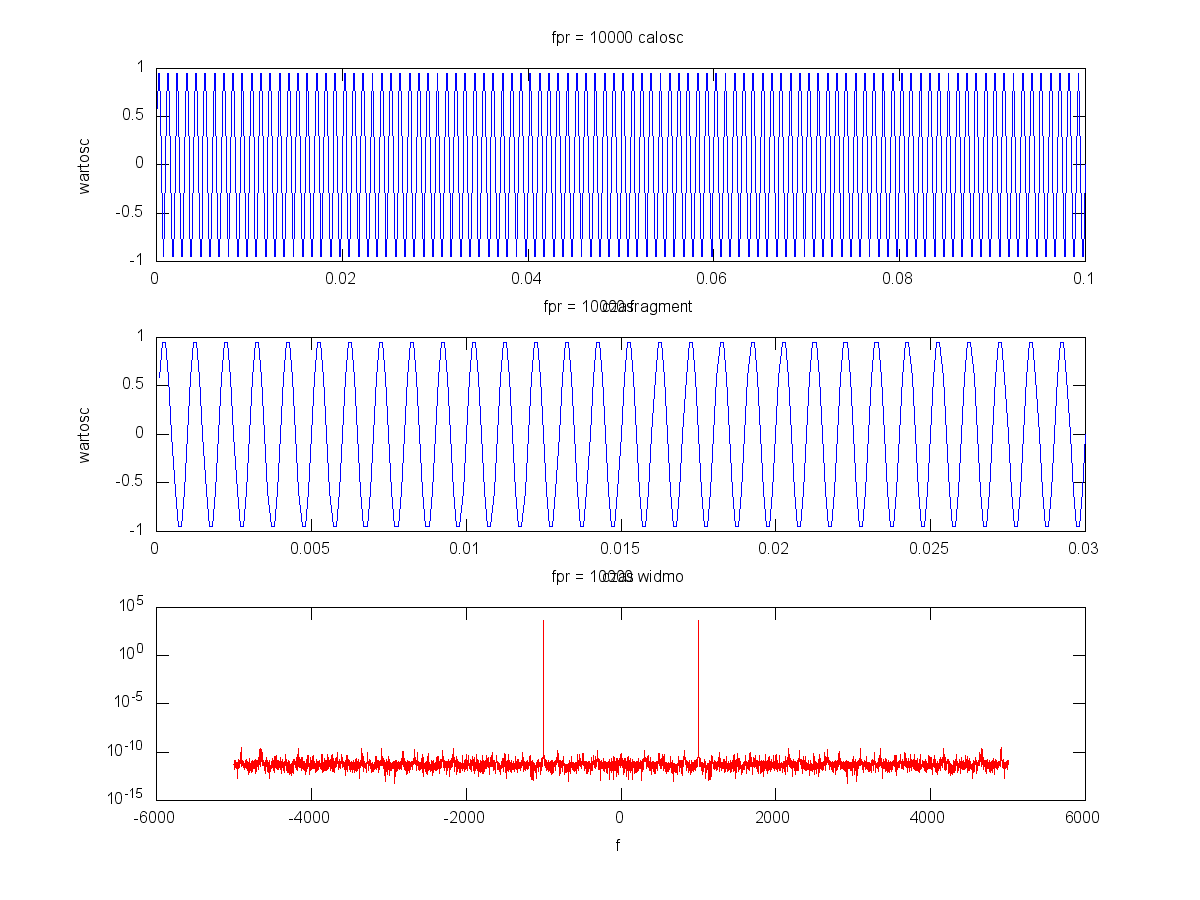
\includegraphics[scale=.5]{out/prob1.png}
	      \caption{\label{prob1} Próbkowanie sygnału sinus, $fpr >> f$}
	    \end{center}
	  \end{figure}
	\end{landscape}

	\begin{landscape}
	  \begin{figure}[htbp]
	    \begin{center}
	      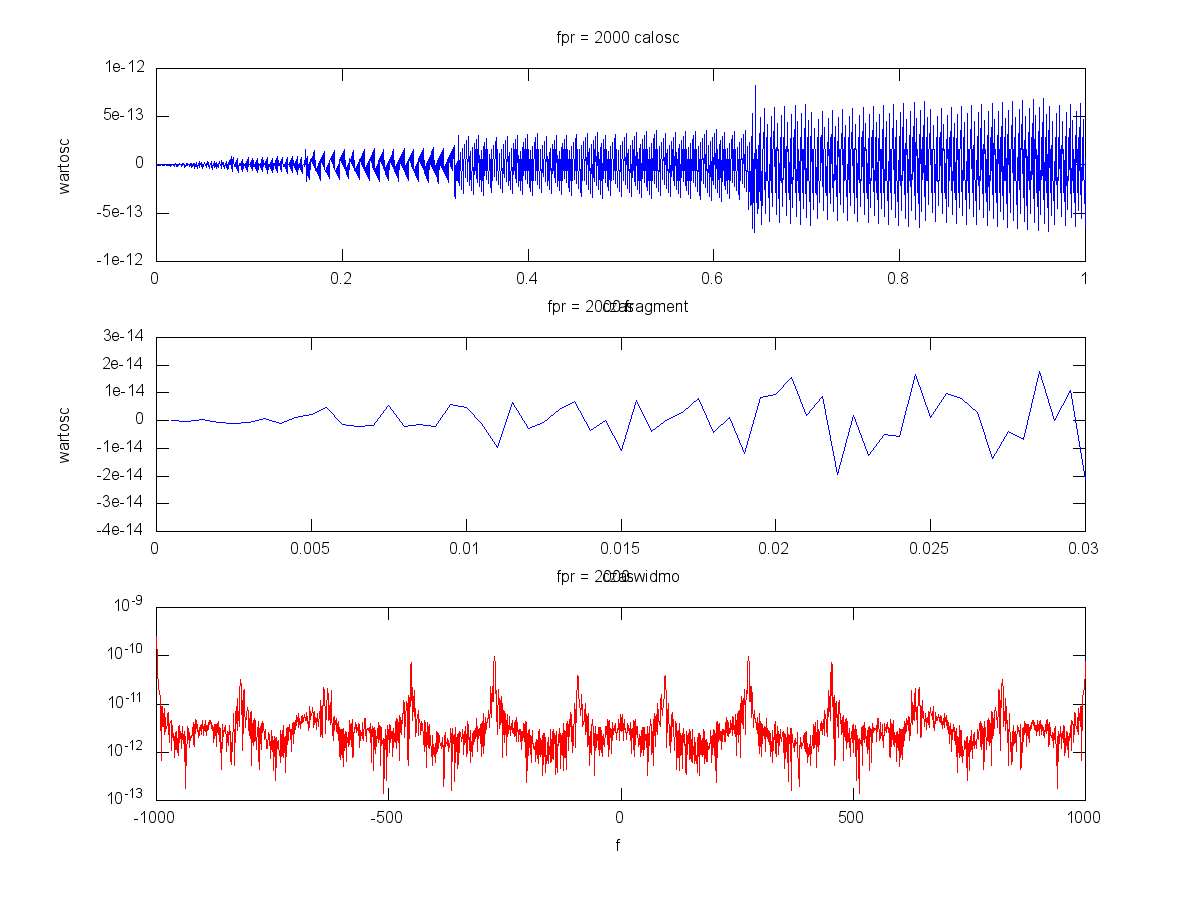
\includegraphics[scale=.5]{out/prob2.png}
	      \caption{\label{prob2} Próbkowanie sygnału sinus, $fpr = 2f$}
	    \end{center}
	  \end{figure}
	\end{landscape}

	\begin{landscape}
	  \begin{figure}[htbp]
	    \begin{center}
	      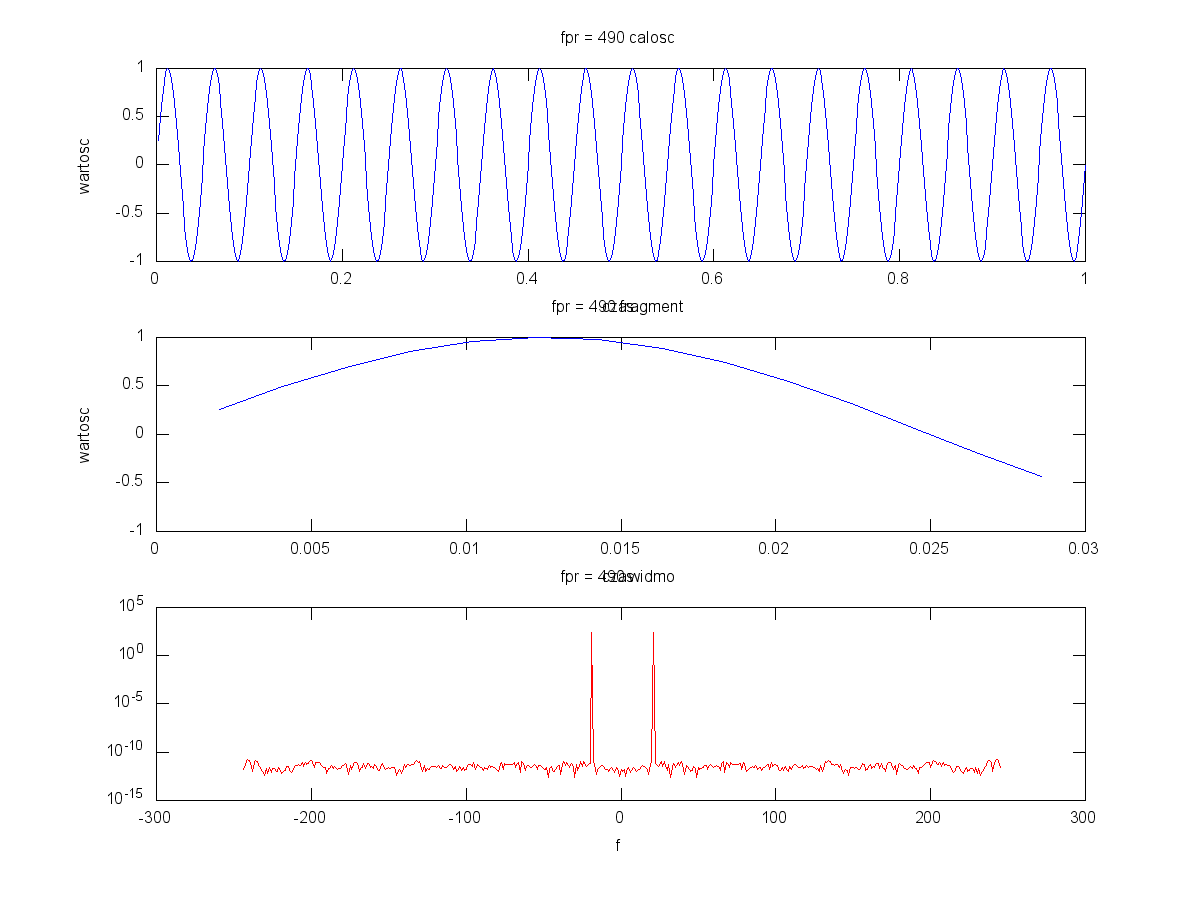
\includegraphics[scale=.5]{out/prob3.png}
	      \caption{\label{prob3} Próbkowanie sygnału sinus, $fpr < f$}
	    \end{center}
	  \end{figure}
	\end{landscape}
	
	
	\begin{landscape}
	  \begin{figure}[htbp]
	    \begin{center}
	      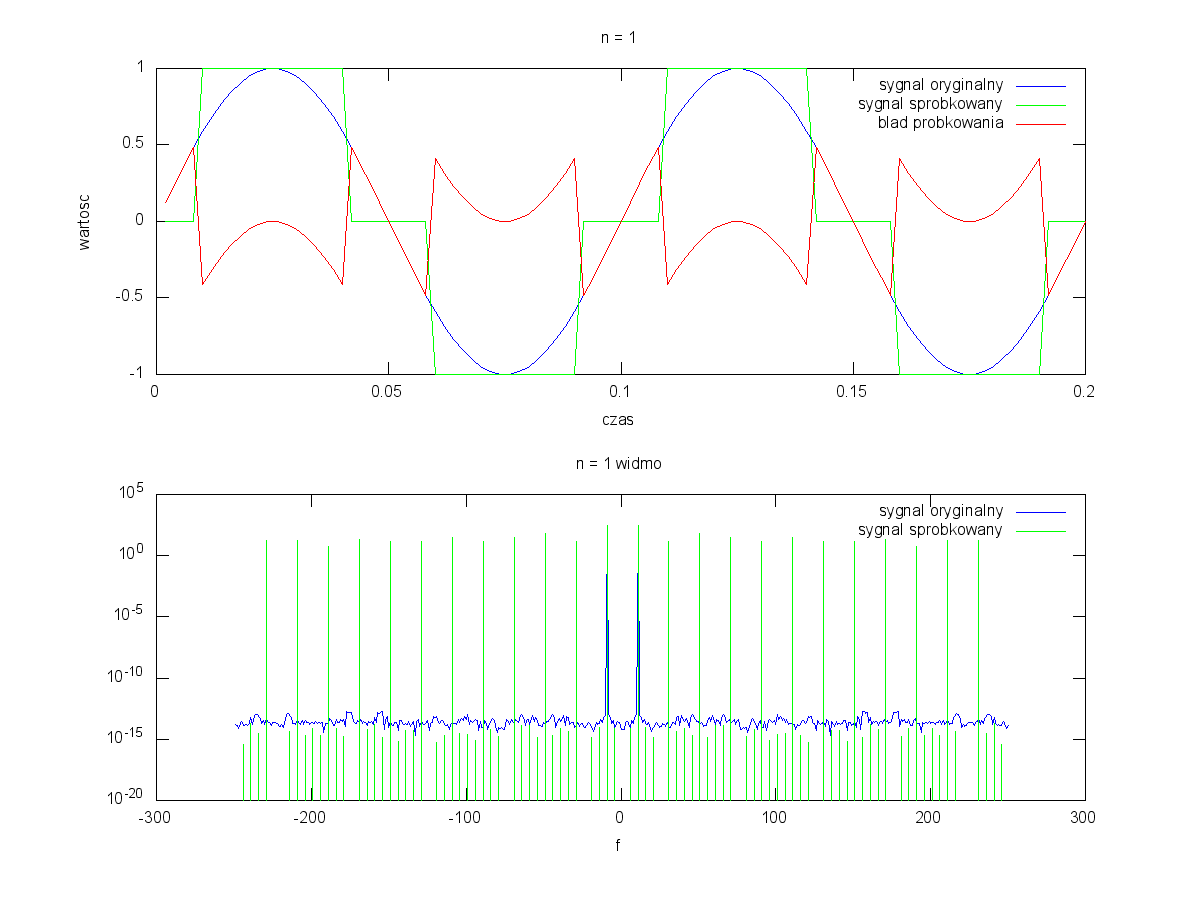
\includegraphics[scale=.5]{out/kwant1-1.png}
	      \caption{\label{kwant1-1} Kwantyzacja sygnału sinus, $n=1$}
	    \end{center}
	  \end{figure}
	\end{landscape}

	\begin{landscape}
	  \begin{figure}[htbp]
	    \begin{center}
	      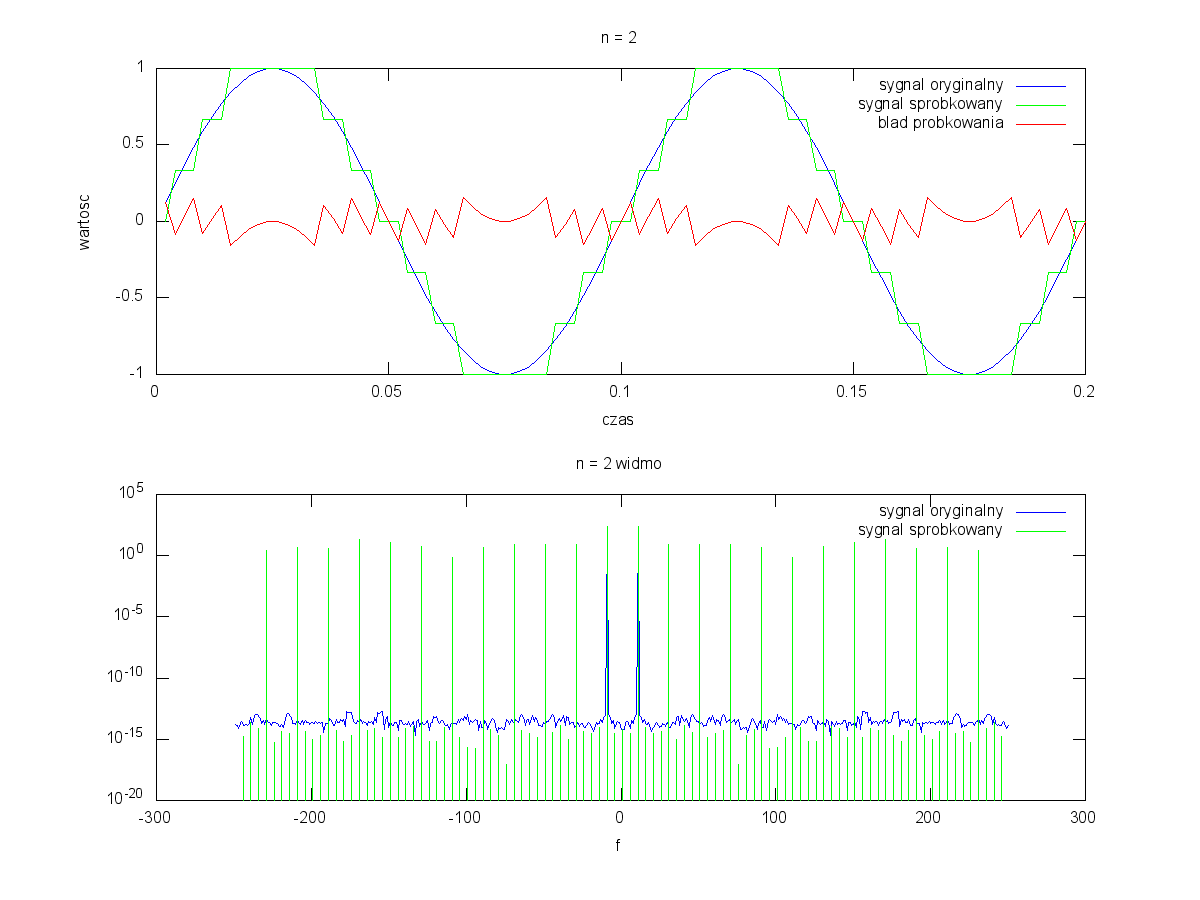
\includegraphics[scale=.5]{out/kwant1-2.png}
	      \caption{\label{kwant1-2} Kwantyzacja sygnału sinus, $n=2$}
	    \end{center}
	  \end{figure}
	\end{landscape}

	\begin{landscape}
	  \begin{figure}[htbp]
	    \begin{center}
	      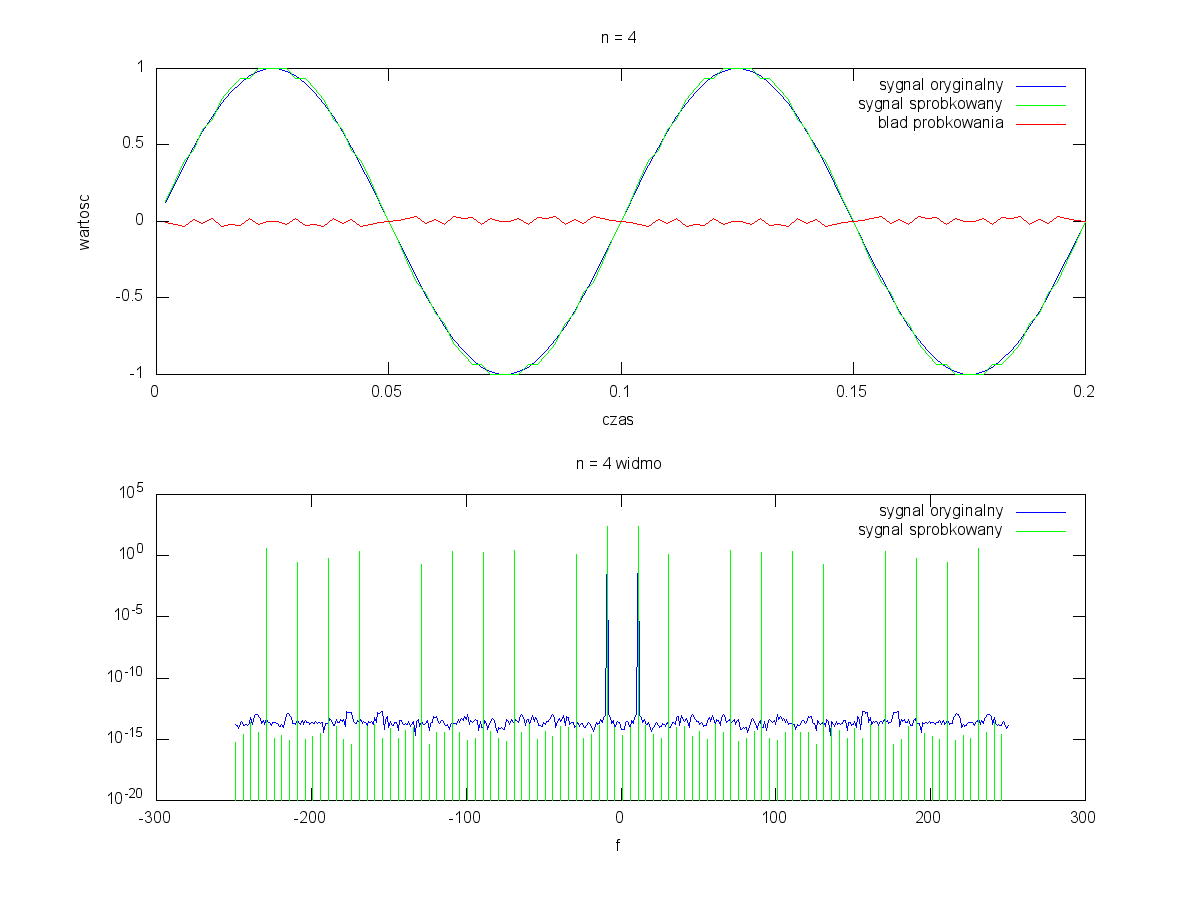
\includegraphics[scale=.5]{out/kwant1-4.png}
	      \caption{\label{kwant1-4} Kwantyzacja sygnału sinus, $n=4$}
	    \end{center}
	  \end{figure}
	\end{landscape}

	\begin{landscape}
	  \begin{figure}[htbp]
	    \begin{center}
	      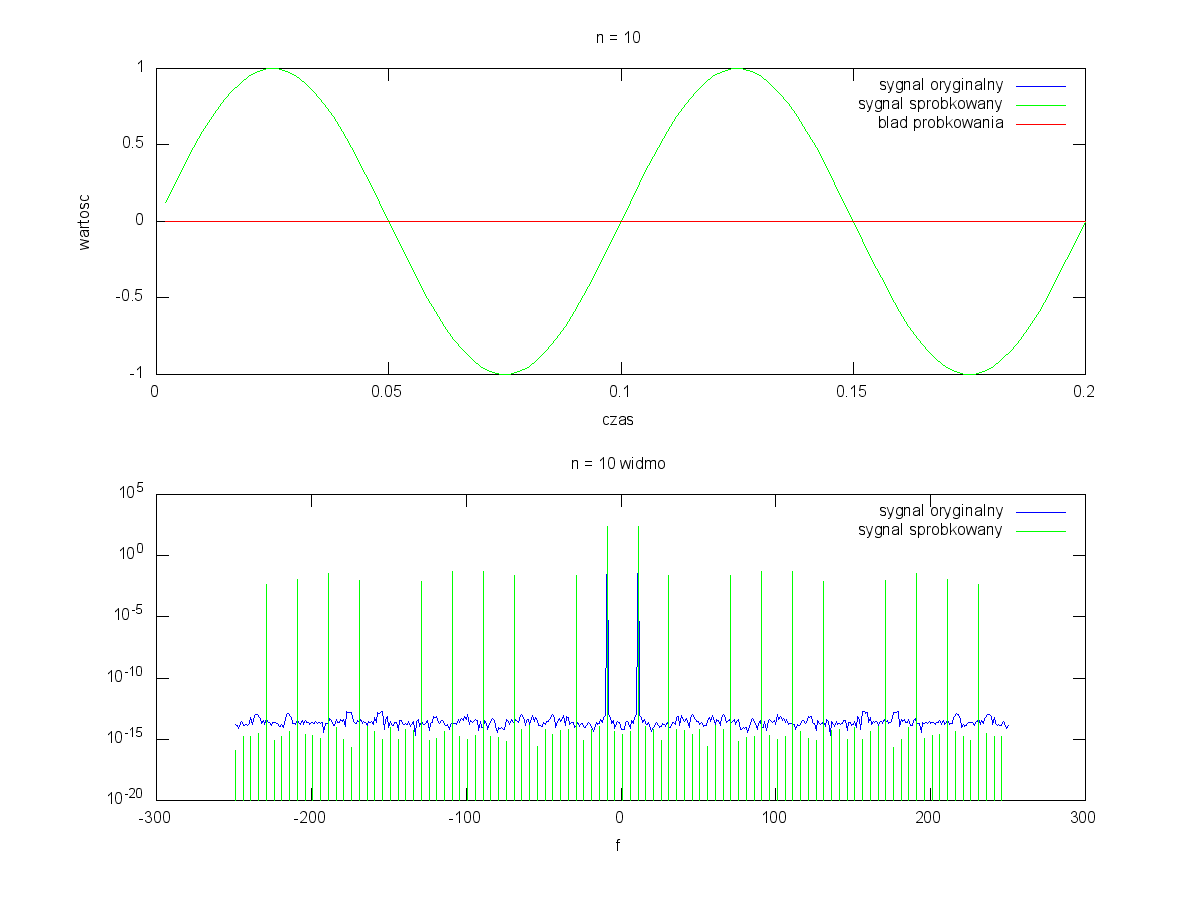
\includegraphics[scale=.5]{out/kwant1-10.png}
	      \caption{\label{kwant1-10} Kwantyzacja sygnału sinus, $n=10$}
	    \end{center}
	  \end{figure}
	\end{landscape}
	
	
	\begin{landscape}
	  \begin{figure}[htbp]
	    \begin{center}
	      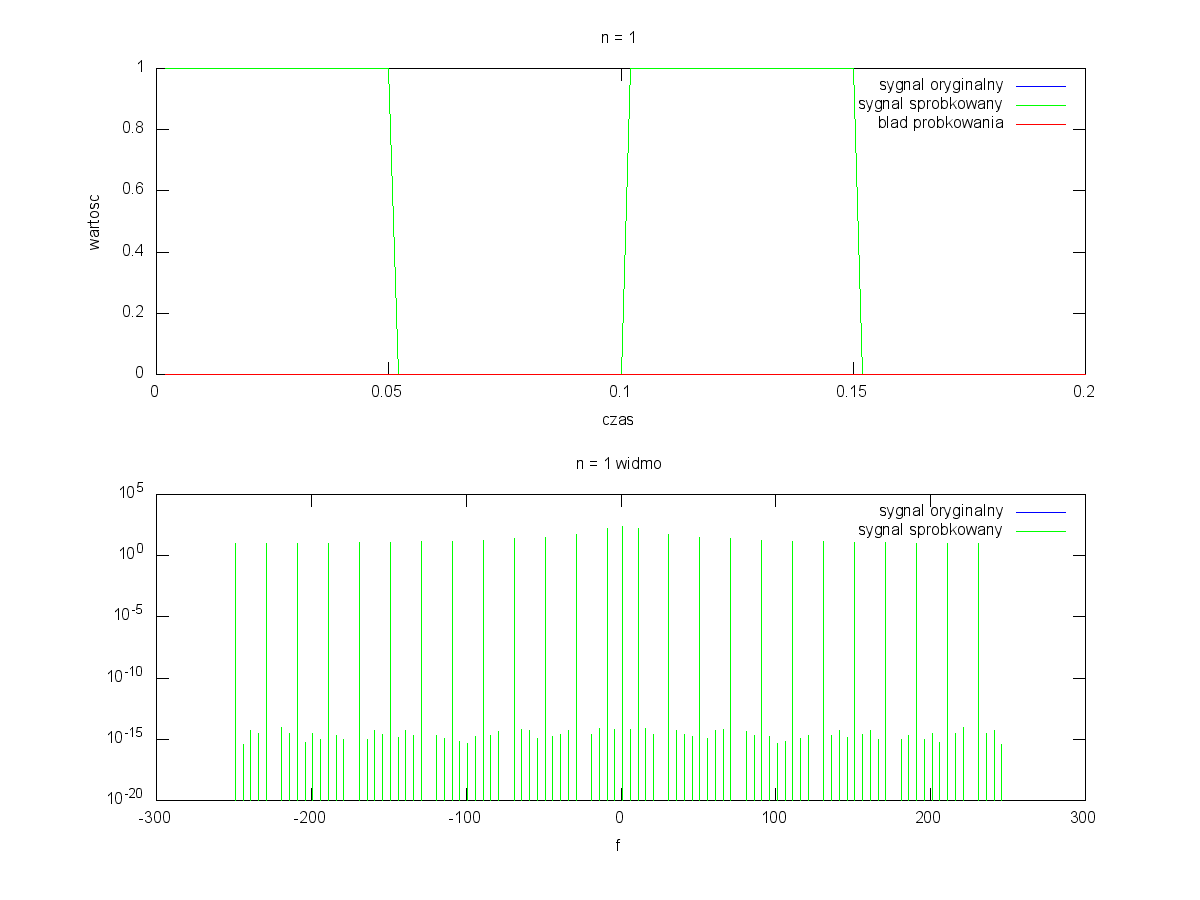
\includegraphics[scale=.5]{out/kwant2-1.png}
	      \caption{\label{kwant2-1} Kwantyzacja sygnału prostokątnego, $n=1$}
	    \end{center}
	  \end{figure}
	\end{landscape}

	\begin{landscape}
	  \begin{figure}[htbp]
	    \begin{center}
	      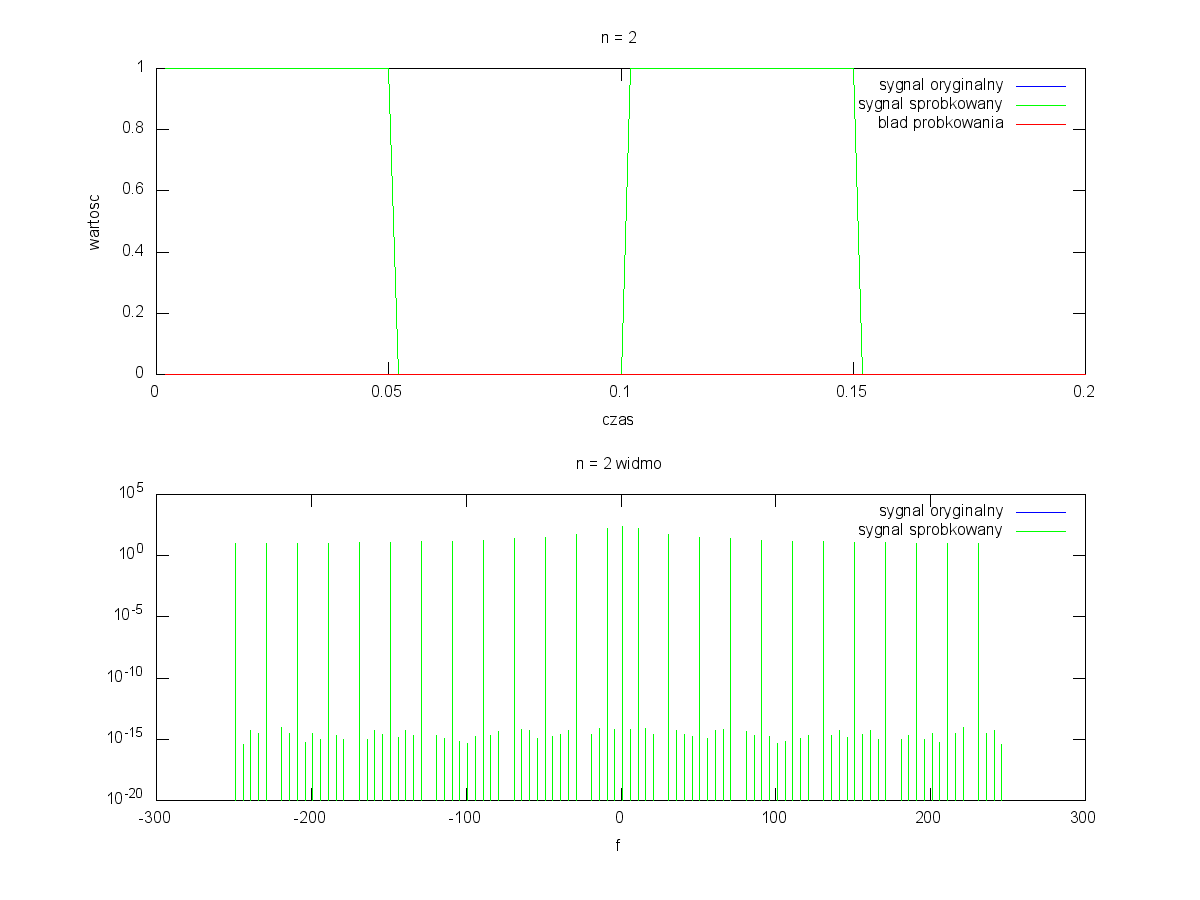
\includegraphics[scale=.5]{out/kwant2-2.png}
	      \caption{\label{kwant2-2} Kwantyzacja sygnału prostokątnego, $n=2$}
	    \end{center}
	  \end{figure}
	\end{landscape}

	\begin{landscape}
	  \begin{figure}[htbp]
	    \begin{center}
	      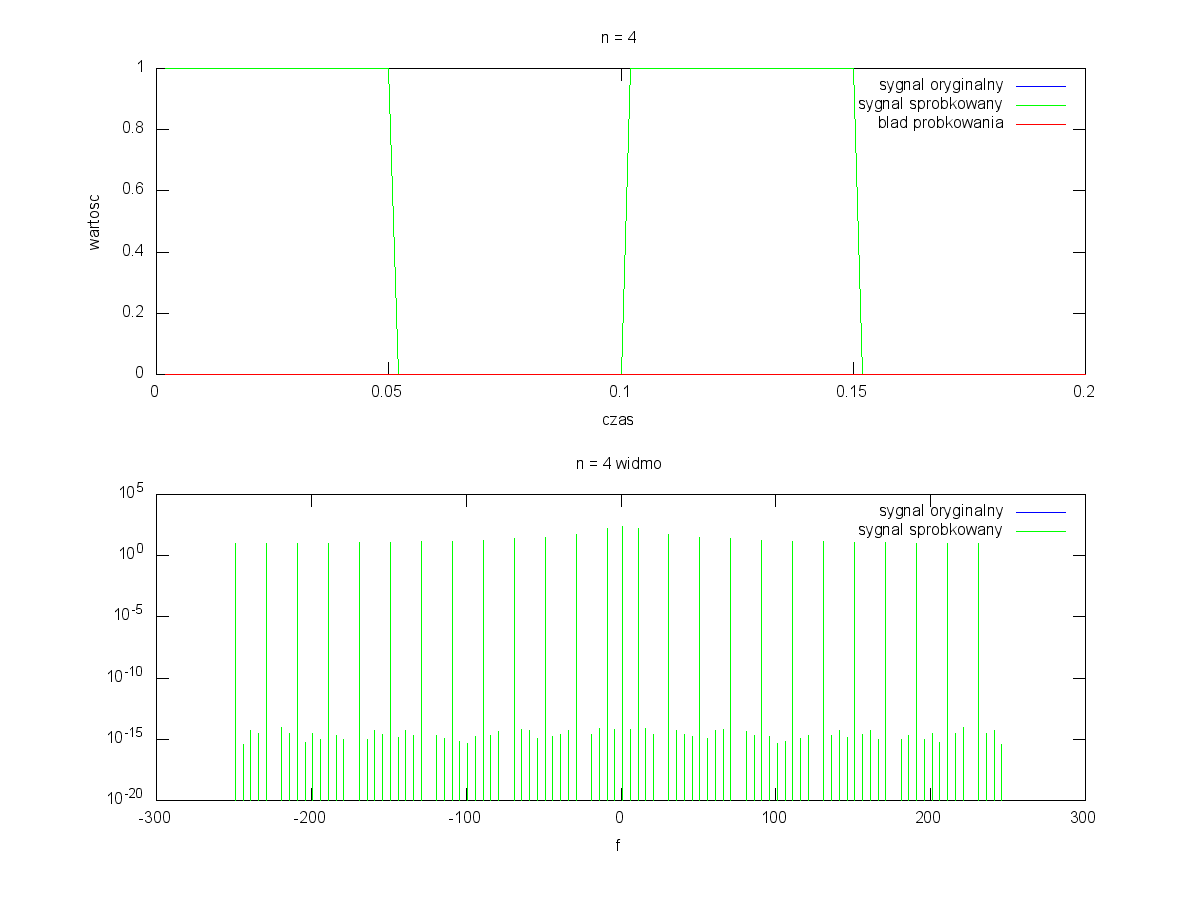
\includegraphics[scale=.5]{out/kwant2-4.png}
	      \caption{\label{kwant2-4} Kwantyzacja sygnału prostokątnego, $n=4$}
	    \end{center}
	  \end{figure}
	\end{landscape}

	\begin{landscape}
	  \begin{figure}[htbp]
	    \begin{center}
	      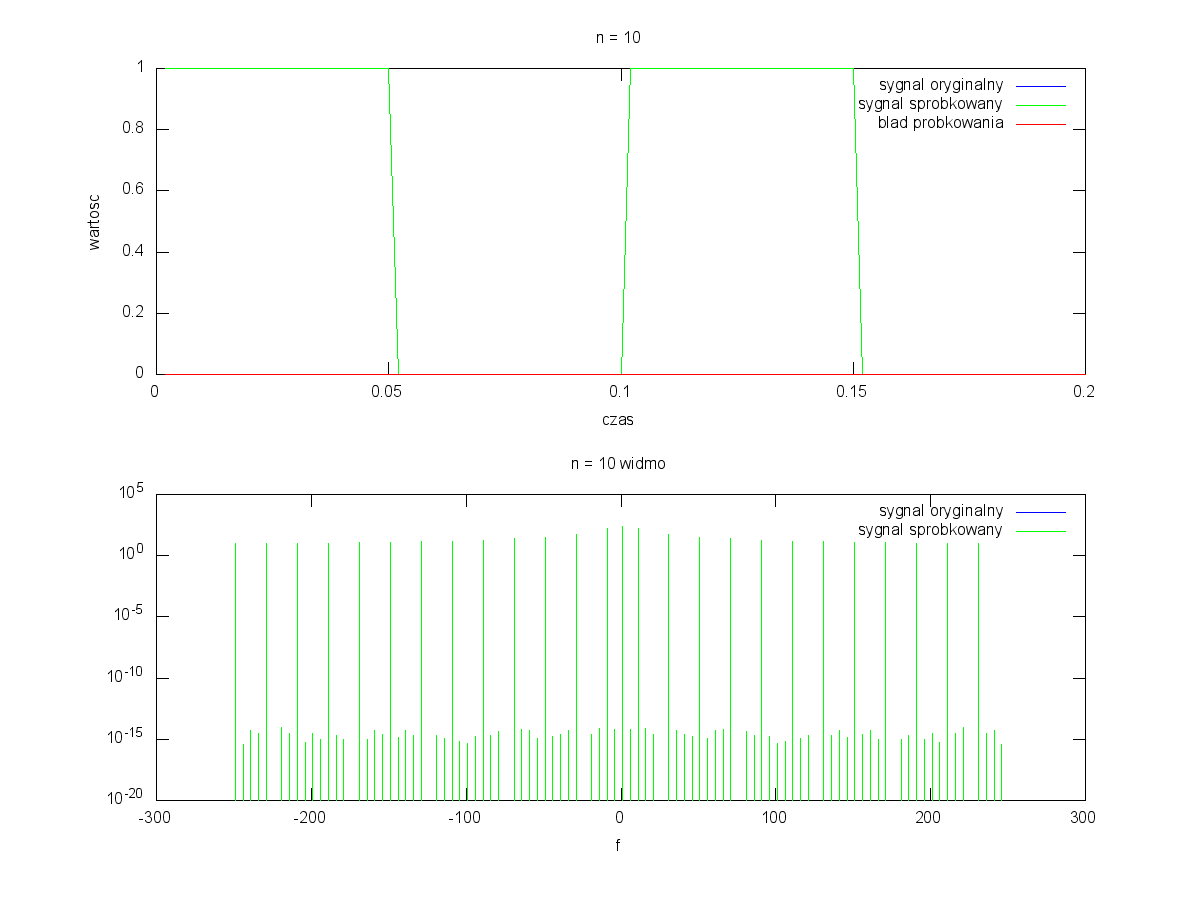
\includegraphics[scale=.5]{out/kwant2-10.png}
	      \caption{\label{kwant2-10} Kwantyzacja sygnału prostokątnego, $n=10$}
	    \end{center}
	  \end{figure}
	\end{landscape}


	\begin{landscape}
	  \begin{figure}[htbp]
	    \begin{center}
	      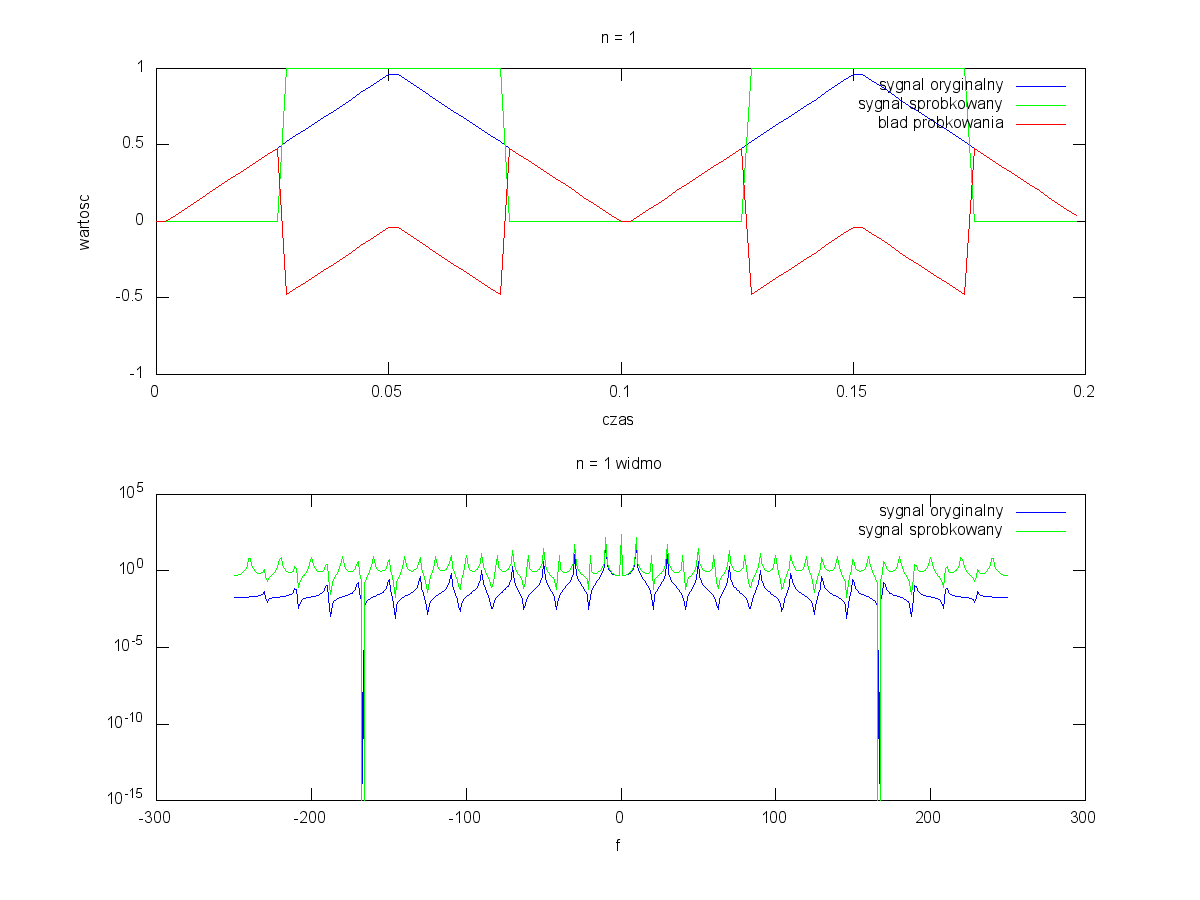
\includegraphics[scale=.5]{out/kwant3-1.png}
	      \caption{\label{kwant3-1} Kwantyzacja sygnału trójkątnego, $n=1$}
	    \end{center}
	  \end{figure}
	\end{landscape}

	\begin{landscape}
	  \begin{figure}[htbp]
	    \begin{center}
	      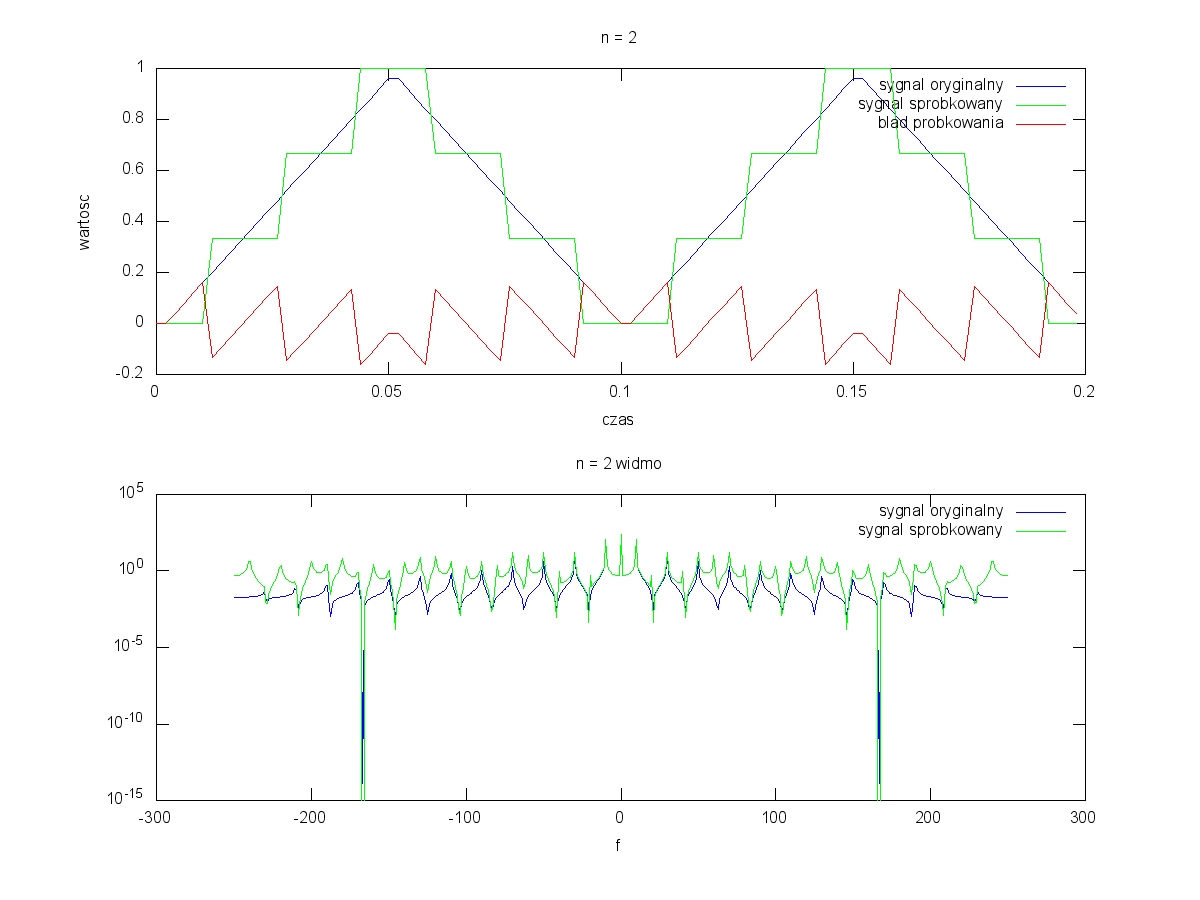
\includegraphics[scale=.5]{out/kwant3-2.png}
	      \caption{\label{kwant3-2} Kwantyzacja sygnału trójkątnego, $n=2$}
	    \end{center}
	  \end{figure}
	\end{landscape}

	\begin{landscape}
	  \begin{figure}[htbp]
	    \begin{center}
	      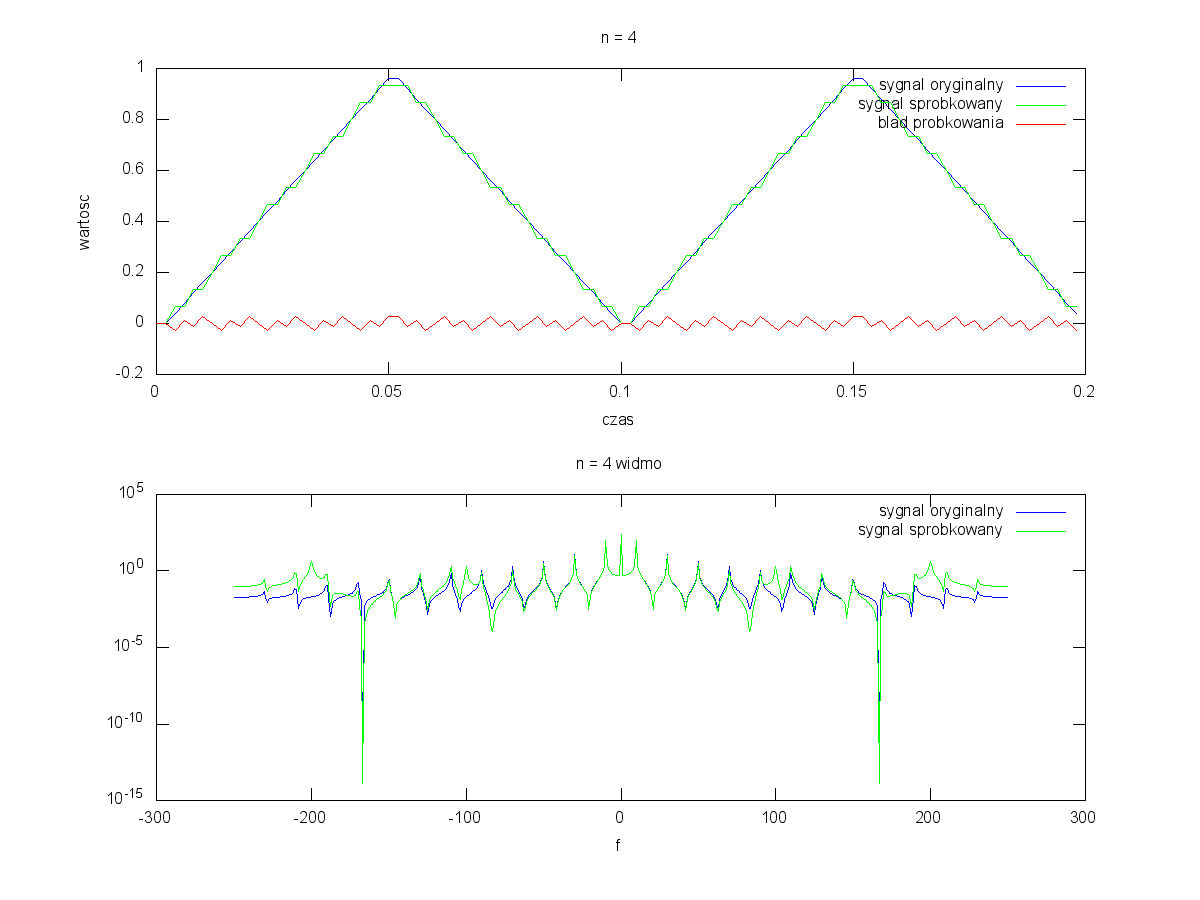
\includegraphics[scale=.5]{out/kwant3-4.png}
	      \caption{\label{kwant3-4} Kwantyzacja sygnału trójkątnego, $n=4$}
	    \end{center}
	  \end{figure}
	\end{landscape}

	\begin{landscape}
	  \begin{figure}[htbp]
	    \begin{center}
	      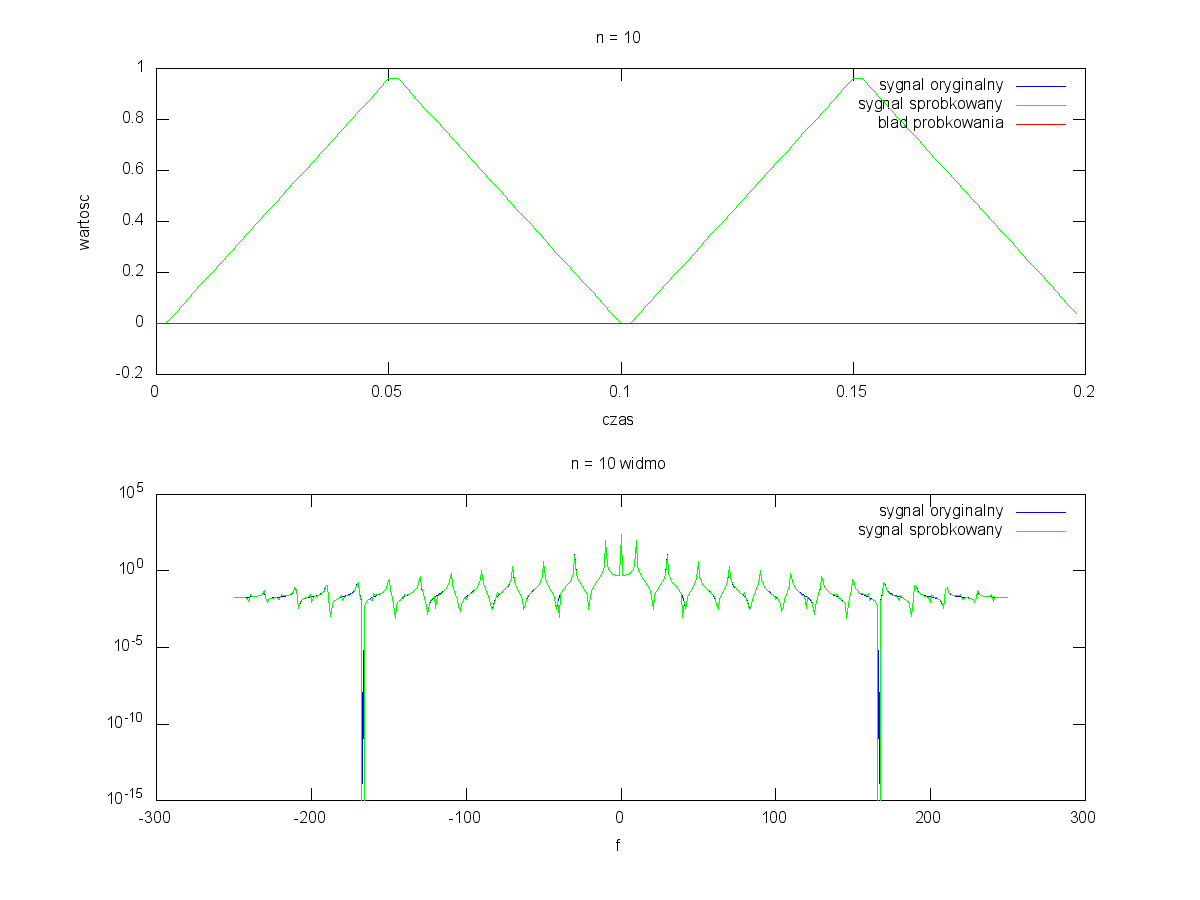
\includegraphics[scale=.5]{out/kwant3-10.png}
	      \caption{\label{kwant3-10} Kwantyzacja sygnału trójkątnego, $n=10$}
	    \end{center}
	  \end{figure}
	\end{landscape}


\end{document}